\documentclass[10pt]{article}
\usepackage[a4paper, tmargin=0.75in, lmargin=0.80in, rmargin=0.80in, bmargin=1in]{geometry}
\usepackage{hyperref}
%\usepackage{multicol}
\hypersetup{
    colorlinks=true,
    linkcolor=black,
    filecolor=magenta,      
    urlcolor=blue,
    citecolor=black,
}
\usepackage{natbib}
\usepackage{graphicx}
\pagestyle{empty}


%%%%%%%%%%%%%%%%%%%%%%%%%%%%%%%%%%%%%%%%%%%%%%%%%%
%%%%%%%%%%%%%%%%%%%%%%%%%%%%%%%%%%%%%%%%%%%%%%%%%%
%%%%%%%%%%%%%%%%%%%%%%%%%%%%%%%%%%%%%%%%%%%%%%%%%%
%%%%%%%%%%%%%%%%%%%%%%%%%%%%%%%%%%%%%%%%%%%%%%%%%%
% ENTER SOME IMPORTANT INFORMATION
%%%%%%%%%%%%%%%%%%%%%%%%%%%%%%%%%%%%%%%%%%%%%%%%%%
%%%%%%%%%%%%%%%%%%%%%%%%%%%%%%%%%%%%%%%%%%%%%%%%%%
%%%%%%%%%%%%%%%%%%%%%%%%%%%%%%%%%%%%%%%%%%%%%%%%%%
%%%%%%%%%%%%%%%%%%%%%%%%%%%%%%%%%%%%%%%%%%%%%%%%%%
\newcommand{\studentname}{Rabbi Hasan}
\newcommand{\studentnumber}{19701071}
%\newcommand{\researchcentre}{Astrophysics Research Centre}
\newcommand{\projecttitle}{rabbihasan.cu@gmail.com}
\newcommand{\supervisor}{Dr Rudra Pratap Deb Nath Sir}
%%%%%%%%%%%%%%%%%%%%%%%%%%%%%%%%%%%%%%%%%%%%%%%%%%
%%%%%%%%%%%%%%%%%%%%%%%%%%%%%%%%%%%%%%%%%%%%%%%%%%
%%%%%%%%%%%%%%%%%%%%%%%%%%%%%%%%%%%%%%%%%%%%%%%%%%
%%%%%%%%%%%%%%%%%%%%%%%%%%%%%%%%%%%%%%%%%%%%%%%%%%
%%%%%%%%%%%%%%%%%%%%%%%%%%%%%%%%%%%%%%%%%%%%%%%%%%
%%%%%%%%%%%%%%%%%%%%%%%%%%%%%%%%%%%%%%%%%%%%%%%%%%

\begin{document}

\begin{center}
{\Huge{Class Diagram}} \\
\vspace{2mm}
{\Large{Dept. of computer science and engineering}} \\
\vspace{1mm}
{\Large{University of Chittagong}}
\end{center}

\vspace{5mm}
\hrule
\vspace{1mm}
\hrule

\vspace{3mm}
\begin{tabular}{ll} 
Name:           	        & {\studentname}   \\ 
ID: 	        & {\studentnumber} \\ 
%Research Centre: 	        & {\researchcentre}  \\ 
Email: 	& {\projecttitle}  \\ 
Submitted to: 	    & {\supervisor}  \\ 
\end{tabular}

\vspace{3mm}
\hrule
\vspace{1mm}
\hrule
%\end{document}

%\begin{document}
\section{Introduction}
% \begin{figure}   
 

 In software engineering, a class diagram in the unified modeling diagram(UML) is a type of static structure diagram that describes the structure of a system by showing the system's classes, their attributes, and the relationships between the classes.
 \vskip18pt%
 \newline
% \newpage
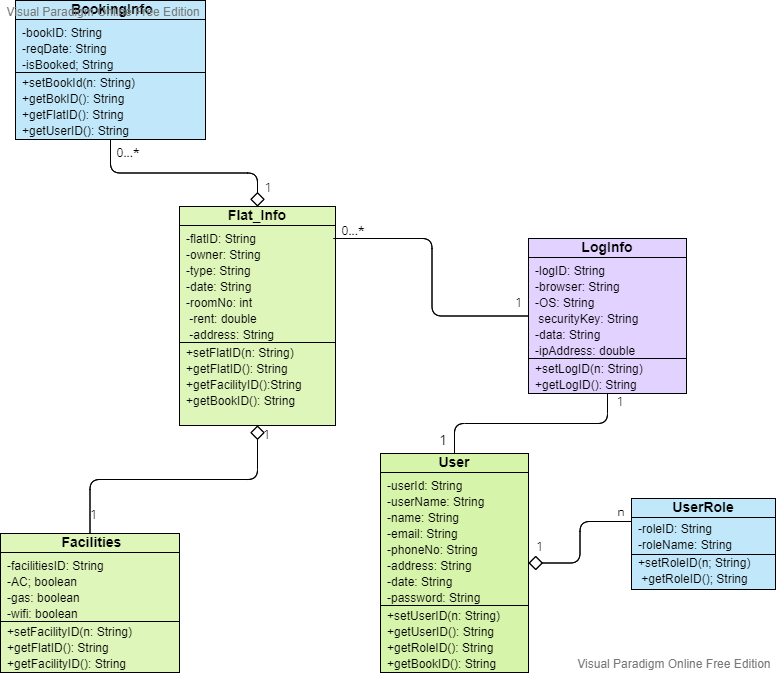
\includegraphics[width=1\textwidth, inner]{Class Diagram Example_ Company Structure (1).png}\\
\begin{center}
 Figure:Class Diagram
\end{center}
 
\newpage
\section{Overview}
The class diagram is the main building block in object oriented modelling. They are being used both for general
conceptual modelling of the systematics of the application, and for detailed modelling translating the models into
programming code. The classes in a class diagram represent both the main objects and or interactions in the
application and the objects to be programmed. In the class diagram these classes are represented with boxes which
contain three parts:
\begin{itemize}
    \item The upper part holds the name of the class.
    \item The middle part contains the attributes of the class.
    \item The bottom part gives the methods or operations the class can take or undertake (exp:- owner : String).
 
\end{itemize}
In the conceptual design of a system, a number of classes are identified and grouped together in a class diagram which helps to determine the statical relations between those objects. With detailed modeling, the classes of the conceptual design are often split in a number of
subclasses.
\vskip10pt%
\noindent
In order to further describe the behavior of systems, these class diagrams can be complemented by state diagram or
UML state machine. Also instead of class diagrams object role modeling can be used if you just want to model the
classes and their relationships.

\section{Relationships}
A relationship is a general term covering the specific types of logical connections found on class and object
diagrams. UML shows the following relationships:
\subsection{External links}
Link is the basic relationship among objects. It is represented as a line connecting two or more object boxes. It can
be shown on an object diagram or class diagram. A link is an instance of an association.In other words, it creates a
relationship between two classes.
\subsection{Association}
An Association represents a family of links. Binary associations (with two ends) are normally represented as a line, with each end connected to a class box. Higher order associations can be
drawn with more than two ends. In such cases, the ends are connected to a central diamond.
\vskip10pt%
\noindent
An association can be named, and the ends of an association can be adorned with role names, ownership indicators,
multiplicity, visibility, and other properties. There are five different types of association. Bi-directional and
uni-directional associations are the most common ones. For instance, a flight class is associated with a plane class
bi-directionally. Associations can only be shown on class diagrams. Association represents the static relationship
shared among the object of two classes.
\subsection{Aggregation}
Aggregation is a variant of the "has a" or
association relationship; aggregation is more specific than association. It is an association
that represents a part-whole or part-of relationship. As a type of association, an
aggregation can be named and have the same adornments that an association can. However, an aggregation may not
involve more than two classes.
\vskip10pt%
\noindent
Aggregation can occur when a class is a collection or container of other classes, but where the contained classes do
not have a strong life cycle dependency on the container—essentially, if the container is destroyed, its contents are
not.
\vskip10pt%
\noindent
In UML, it is graphically represented as a hollow diamond shape on the containing class end of the tree of lines that
connect contained class(es) to the containing class.
\vskip18pt%

% \newpage
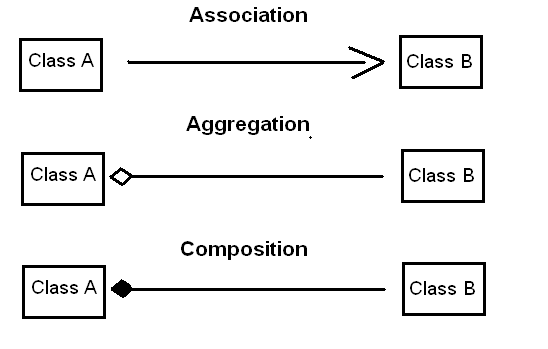
\includegraphics[width=1\textwidth,height=0.30\textheight ,inner]{bfBSY.png}\\
\begin{center}
 Figure:Relationships: 1. Association, 2. Aggregation and 3. Composition. 
\end{center}
\subsection{Composition}
Composition is a stronger variant of the "owns a” or association
relationship; composition is more specific than aggregation. It is represented with a solid diamond shape. 
\vskip10pt%
\noindent
Composition usually has a strong life cycle dependency between
instances of the container class and instances of the contained class(es): If the container is destroyed, normally every instance that it contains is destroyed as well. Note that a part can (where allowed) be removed from a composite before the composite is deleted, and thus
not be deleted as part of the composite.
\vskip10pt%
\noindent
The UML graphical representation of a composition relationship is a filled diamond shape on the containing class
end of the tree of lines that connect contained class(es) to the containing class.
\vskip10pt%
\centering
[link: https://www.yumpu.com/en/document/read/36058323/class-diagram-umlpdf]
\
%\section{Research Plan}
%In this section, please outline the short- and long-term goals of the research. These can be stipulated as bullet points. This section should be approximately 0.5 -- 1.0 pages long. For example, you can refer the reader to Section~{\ref{sec:shorttermgoals}} for your short-term goals, and Section~{\ref{sec:longtermgoals}} for your long-term goals.

%\subsection{Short-term Goals}
%\label{sec:shorttermgoals}
%My immediate short-term goals are outlined below.
%\begin{enumerate}
%    \item Short-term goal 1.
 %   \item Short-term goal 2.
 %   \item Short-term goal 3.
%\end{enumerate}

%\subsection{Long-term Goals}
%\label{sec:longtermgoals}
%The project's long-term goals are outlined below.
%\begin{enumerate}
 %   \item Long-term goal 1.
  %  \item Long-term goal 2.
   % \item Long-term goal 3.
%\end{enumerate}



%\bibliographystyle{aasjournal}
%\bibliography{references}{}

 

\end{document}
